\section{Equicontinuity}

\begin{frame}
	\begin{definition}[Topological Dynamical System (TDS)]
		Let $(X, d)$ be a \textbf{compact} metric space and $T$ a topological group. Let there be a group action $T \times X \to X$ ($ex = x$ and $s(tx) = (st)x$ for all $s, t \in T$, $x \in X$), which is continuous. Then we call the pair $(X, T)$ a \textbf{topological dynamical system} (TDS).
	\end{definition}
	\begin{remark}
		Note that for each $t \in T$ the map $x \mapsto tx$ is a homeomorphism.
	\end{remark}
	\begin{remark}
		Let $\alpha: X \to X$ be a homeomorphism. Then this gives rise to a $\mathbb{Z}$ action with $nx := \alpha^n(x)$ for $n \in \mathbb{Z}$. In this case we write $(X, \alpha)$ for this dynamical system.
	\end{remark}
	\begin{definition}[Minimal TDS]
		A TDS $(X, T)$ is minimal if for every $x \in X$ the orbit $\{tx, t \in T\}$ is dense in $X$.
	\end{definition}
\end{frame}

\begin{frame}
	\begin{definition}[Factors and Isomorphisms]
		A TDS $(Y, T)$ is a \textbf{factor} of $(X, T)$ if there exists a \textbf{factor map}, i.e. a surjective and continuous map
		\begin{align*}
			\pi: X \to Y
		\end{align*}
		such that $\pi(tx) = t\pi(x)$ for all $t \in T,\ x \in X$.
		
		A factor map is an \textbf{isomorphism} (of TDS) if it is a homeomorphism.
		
		Two TDS are isomorphic if there exists an isomorphism between them.
	\end{definition}
	\begin{definition}[ICER]
		An \textbf{invariant closed equivalent relation} (ICER) $R \subseteq X \times X$ is a equivalence relation, such that $R$ is closed and $tR = R$.
		
		Then $X/R$ becomes a TDS with $t[x] := [tx]$ for all $t \in T$ and $x \in X$.
	\end{definition}
\end{frame}

\begin{frame}
	\begin{proposition}
		Let $R \subseteq X \times X$ be an ICER. Then we can define a factor by
		\begin{align*}
			\pi_R: X \to X/R \quad \pi_R(x) := [x] \quad \forall x \in X.
		\end{align*}
	
		Let $\pi: X \to Y$ be a factor map. Then we can define an ICER by
		\begin{align*}
			R_\pi := \{(x, y) \in X \times X;\ \pi(x) = \pi(y)\}.
		\end{align*}
	
		In this case we have $(Y, T) \cong (X/R_\pi, T)$.
	\end{proposition}
	\begin{definition}[Conjugated and Equivalent factors]
		Let $(Y, T)$ and $(Z, T)$ be two factors of $(X, T)$ with factor maps $\pi$ and $\rho$.
		
		The factors are \textbf{conjugated} if $(Y, T) \cong (Z, T)$.
		
		The factors are \textbf{equivalent} if $R_\pi = R_\rho$. In this case they are also conjugated.
	\end{definition}
\end{frame}

\begin{frame}
	\begin{definition}[Equicontinuous TDS]
		The TDS $(X, T)$ is \textbf{equicontinuous} if for $\varepsilon > 0$ there is some $\delta > 0$ such that
		\begin{align*}
			d(x, y) < \delta \Rightarrow d(tx, ty) < \varepsilon
		\end{align*}
		for all $x, y \in X$ and $t \in T$.
	\end{definition}
	\begin{remark}
		Intuitively equicontinuity means that two points that are close, were and will be always close.
	\end{remark}
	\begin{proposition}
		Let $d, \tilde{d}$ be two metrics on $X$, that induce the same topology. Then $(x, T)$ is equicontinuous with respect to $d$ if and only if it is equicontinuous with respect to $\tilde{d}$.
	\end{proposition}
	\begin{proposition}
		Equicontinuity is preserved under isomorphisms and (countable) products. 
	\end{proposition}
\end{frame}

\begin{frame}
	\frametitle{Example: Circle Rotations}
	\begin{columns}
		\begin{column}{0.5\textwidth}
			We look at the circle $\mathbb{S} := \mathbb{R}/\mathbb{Z}$ (identify $[x] = x + \mathbb{Z}$ for $x \in \mathbb{R}$ with $e^{2\pi ix}$ in $\mathbb{C}$). The metric on $\mathbb{S}$ is given by
			\begin{align*}
				d_\mathbb{S}([x], [y]) := \min_{n \in \mathbb{Z}} |x - y + n|.
			\end{align*}
			
			\medskip			
			Fix $a \in \mathbb{R}$ and define
			\begin{align*}
				\alpha([x]) := [x + a].
			\end{align*}
			
			\medskip
			The TDS $(\mathbb{S}, \alpha)$ is minimal iff $a \notin \mathbb{Q}$.
			
			\medskip
			We have for $[x], [y] \in \mathbb{S}$ and $n \in \mathbb{Z}$ that
			\begin{align*}
				d_\mathbb{S}(\alpha^n([x]), \alpha^n([y])) = d_\mathbb{S}([x], [y]),
			\end{align*}
			i.e. $\alpha$ is isometric. Equicontinuity is an immediate consequence.
		\end{column}
		\begin{column}{0.5\textwidth}
			\begin{figure}[h]
				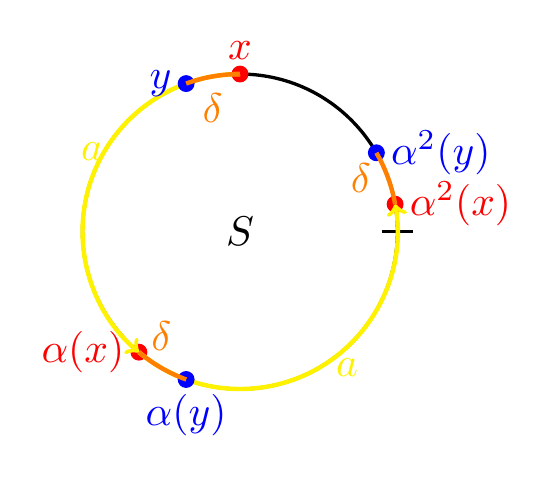
\begin{tikzpicture}
					\draw[very thick] (0, 0) circle (2) node[scale=1.5] {$\mathbb{S}$};
					\draw[very thick] (1.8, 0) -- (2.2, 0);
					
					\filldraw[color=red] (0, 2) circle (.1) node[anchor=south, scale=1.5] {$x$};
					\filldraw[color=red] (-1.284, -1.532) circle (.1) node[anchor=east, scale=1.5] {$\alpha(x)$};
					\filldraw[color=red] (1.970, .347) circle (.1) node[anchor=west, scale=1.5] {$\alpha^2(x)$};
					
					\draw[ultra thick, color=yellow, ->] (0, 2) arc (90:230:2) node[above, midway, scale=1.5] {$a$};
					\draw[ultra thick, color=yellow, ->] (-1.284, -1.532) arc (230:370:2) node[right, midway, scale=1.5] {$a$};
					
					\filldraw[color=blue] (-0.684, 1.879) circle (.1) node[anchor=east, scale=1.5] {$y$};
					\filldraw[color=blue] (-0.684, -1.879) circle (.1) node[anchor=north, scale=1.5] {$\alpha(y)$};
					\filldraw[color=blue] (1.732, 1) circle (.1) node[anchor=west, scale=1.5] {$\alpha^2(y)$};
					
					\draw[ultra thick, color=orange] (0, 2) arc (90:110:2) node[below, midway, scale=1.5] {$\delta$};
					\draw[ultra thick, color=orange] (-1.284, -1.532) arc (230:250:2) node[above, midway, scale=1.5] {$\delta$};
					\draw[ultra thick, color=orange] (1.970, .347) arc (10:30:2) node[left, midway, scale=1.5] {$\delta$};
				\end{tikzpicture}
			\end{figure}
		\end{column}
	\end{columns}
\end{frame}
